\section{Results}
\subsection{Implementation of the TEBD algorithm}

%4.1a
\subsubsection{Implementation of the $\ket{\uparrow\uparrow\cdots\uparrow}$ state}
We generated an instance of the MPS class using the \texttt{init\_spinup\_MPS()} function which is given in the file \texttt{a\_mps.py}. This function returns a product state of all spin ups as an MPS, and takes as an argument the length of the chain $L$. We set $L = 14$. We then define the \textit{Pauli matrices} as $2\times 2$ matrices with the following forms:
\begin{align*}
\sigma^x &=
\begin{pmatrix}0&1\\1&0\end{pmatrix}
\\
\sigma^y &=
\begin{pmatrix}0&-i\\i&0\end{pmatrix} 
\\
\sigma^z &=
\begin{pmatrix}1&0\\0&-1\end{pmatrix} .
\end{align*}
Using the function \texttt{site\_expectation\_value()}, which takes a matrix as an input, we obtain the site expectation values for the $\sigma^x$ and the $\sigma^z$ operators. For the $\sigma^x$ operators, the expectation values for all sites are zero, while for the $\sigma^z$ operator the expectation values for all sites are one. This, of course, matches what we expect for the $\ket{\uparrow\uparrow\cdots\uparrow}$ state.

%4.1b
\subsubsection{Implementation of the $\ket{\rightarrow\rightarrow\cdots\rightarrow}$ state}
We wrote the function \texttt{init\_plus\_MPS} which returns a product state of $\ket{\rightarrow}^{\otimes L} = \left( \frac{1}{\sqrt{2}} \left( \ket{\uparrow} + \ket{\downarrow} \right) \right) ^{\otimes L}$ for a given length of chain $L$. We once again set $L = 14$. We checked the expectation values of the Pauli matrices in the same way as for the $\ket{\uparrow\uparrow\cdots\uparrow}$ state. This time, we obtain the expectation values $0$ on all sites for the operator $\sigma^z$, while for the $\sigma^x$ state we get the expectation values of 1. This matches the expected expectation values for the $\ket{\rightarrow\rightarrow\cdots\rightarrow}$ state.

%4.1c
\subsubsection{Energies of the $\ket{\uparrow}^{\otimes L}$ and $\ket{\rightarrow}^{\otimes L}$ states in the transverse field Ising model}
Using the previously defined functions, we generate two instances of the MPS class which correspond to the states $\ket{\uparrow}^{\otimes L}$ and $\ket{\rightarrow}^{\otimes L}$ for $L = 14$. Using the \texttt{TFIModel()} and \texttt{energy()} functions from the file \texttt{b\_model.py}, we calculate the energies of these 2 states in the transverse field Ising model \ref{eq:TFI}. In this case, the longitudinal field $h$ is turned off, which is equivalent to setting $h=0$ in \ref{eq:TFI}. We used $J = 1$ and $g\in\{0.5, 1, 1.5\}$. The energies are given on the figure \ref{fig:energy_comparison} as a function of the transverse-field strength $g$. We can see that for the $\ket{\uparrow}^{\otimes L}$ state, the energy decreases with the increasing transverse field, while for the $\ket{\rightarrow}^{\otimes L}$ state the energy is independent from the transverse field strength. This is in accordance to what we expect, as the transverse field is aligned with the $\ket{\uparrow}$ state, and orthogonal to the $\ket{\rightarrow}$ state.

%4.1d
\subsubsection{Ground state energy of the transverse field Ising model}
For the same values of $g$ and $J$ we find the ground-state energy of the TFI model, which is also plotted on \ref{fig:energy_comparison}. We used the function \texttt{example\_TEBD\_gs\_finite()} from \texttt{c\_tebd.py} to do this. We see that the energy of the ground state is lower than both the energies of the $\ket{\uparrow}^{\otimes L}$ and of the $\ket{\rightarrow}^{\otimes L}$ states. This makes sense, as the ground state has the lowest energy by definition. Additionally, we see that as $g$ increases, the energy of the state $\ket{\uparrow}^{\otimes L}$ approaches the ground state energy. This makes sense, as with the increasing field, the spins will tend to align with the field more, matching the $\ket{\uparrow}^{\otimes L}$ and $\ket{\downarrow}^{\otimes L}$ states. In actuallity, as $|g|\rightarrow\infty$, the ground states of the TFI model will approach those 2 states (they are degenerate ground states in that case).


\begin{figure}
    \ve
    \centering
    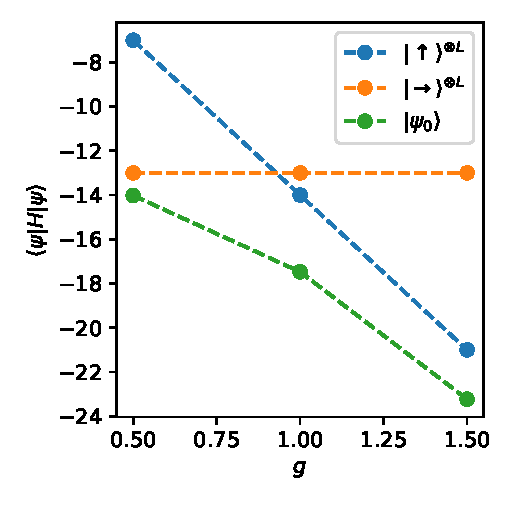
\includegraphics[width=0.8\linewidth]{LaTeX/Plots/energy_comparison.pdf}
    \caption{Energy of the $\ket{\uparrow}^{\otimes L}$ (blue), $\ket{\rightarrow}^{\otimes L}$ (orange) and ground (green) state of the TFI model as a function of the transverse field strength $g$}
    \label{fig:energy_comparison}
\end{figure}

\subsection{Ground state Phase diagram}

%4.2a
\subsubsection{Correlations function}
We define the function \texttt{correlations()}, which takes as an argument an instance of the \texttt{MPI()} class, two operators $X$ and $Y$, and an integer $i$. It returns an array of correlations $\braket{\psi|X_i Y_j|\psi}$ for all $L>j\geq i$, where $L$ is the length of the chain.

%4.2b
\subsubsection{Correlations in the TFI model}
We initialize the system in the $\ket{\uparrow}^{\otimes L}$ state for $L=30$. Using the function \texttt{example\_TEBD\_gs\_finite()} we let the system evolve to the ground state for different values of g. Then, on the ground state, we execute the function \texttt{correlations()} to find $\braket{\sigma^x_{8}\sigma^x_{j}}$ for $j \in \{8, 9, \dots, 30\}$. We plot these correlations as a function of $j$ and for different values of $g$ on figure \ref{fig:correlations}. We can see that for a fixed $g$ the correlation between sites $8$ and $j$ decreases as $j$ increases. This makes intuitive sense, as the further away the 2 sites are, the less correlated they will be. Secondly, we see that with increasing $g$ the correlation between sites $8$ and $j$ decreases for a constant index $j$. This also makes sense because as the transverse field strength increases, the less the interactions between the neighboring sites are of note.\\\\
Another interesting observation is that for values $g<1$ the correlations seem to approach a constant value as $j$ increases (ignoring boundary effects), while for the case of $g>1$ they exponentially approach 0. At the value $g=1$, the correlations seem to obey a power-law decay, indicating the presence of a phase transition. 
\begin{figure}
    \ve
    \centering
    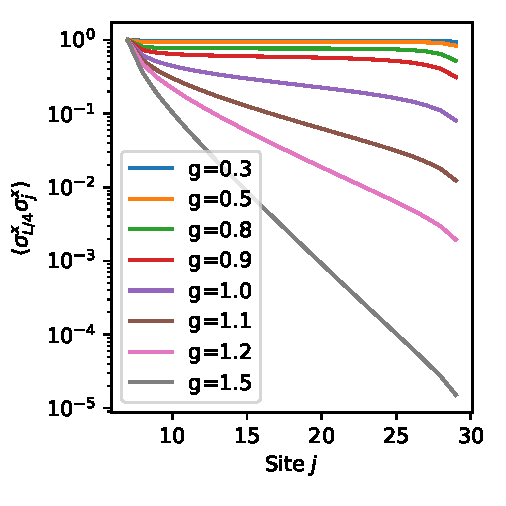
\includegraphics[width=0.8\linewidth]{LaTeX/Plots/correlations.pdf}
    \caption{Correlations between sites $L./4 = 7$ and $j$ for different transverse field strengths $g$}
    \label{fig:correlations}
\end{figure}
%4.2c
\subsubsection{Magnetization in the TFI model}
We define magnetization as the limit
\begin{equation}
    \braket{\sigma^x_i \sigma^x_j} \rightarrow m^2 \,\text{for}\,|i-j|\rightarrow \infty
\end{equation}
For the same values of $g$ we estimate magnetization $m$ as
\begin{equation}
    m = \sqrt{\braket{\sigma^x_7 \sigma^x_{26}}}.
\end{equation}
We do not use the last few indices in the chain in order to avoid boundary effects. We plot $m$ against $g$ on \ref{fig:magnetization}. We can clearly see that there is a phase transition in the order parameter $m$ at $g = 1$, which matches what we have concluded previously. If the length of the chain $L$ that we looked at was greater, this transition would be even sharper.
\begin{figure}
    \centering
    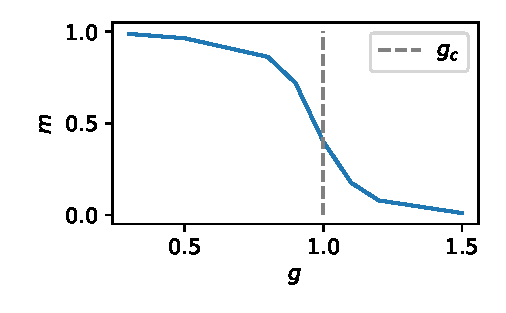
\includegraphics[width=0.8\linewidth]{LaTeX/Plots/magnetisation.pdf}
    \caption{Magnetization $m$ as a function of $g$ for the TFI model}
    \label{fig:magnetization}
\end{figure}





\subsection{The Dynamic Structure Factor}
Next part of the task required of us to study the correlations, entanglement structrure and spectral properties of the TFI model. We began by creating a function that calculates correlations of the form
\begin{equation}
    C(t, j) = \bra{\psi_0} e^{i H t} \sigma_j^y e^{- i H t}\sigma_{L/2}^y \ket{\psi_0}.\label{CorrelationEquation}
\end{equation}
This would physically match causing a perturbation on the ground state in the middle of the chain at $t=0$, and seeing how the said perturbation evolves along the chain as a function of time $t$. In that sense, the procedure can be seen as a local quench.
This function can then be used to obtain the spectral properties of the system. 
Like in the first part of the report, we obtain the ground state of the TFI model $\ket{\psi_0}$ by performing an imaginary time evolution, using the TEBD algorithm. 
\\\\
We are particularly interested in the differences between the symmetric and
symmetry-broken phases ($g<1$ and $g>1$). For each choice of parameters $g$, $J$,
and $h$, we have to choose appropriate simulation times $T$ and system sizes $L$,
such that the spread of correlations does not cause finite-size boundary effects.
Our choices of parameters are listed in table \ref{DSF_Table}.
The results for all of the cases are shown on \ref{fig:4c_g_0_2}, \ref{fig:4d_g_0_2}
and \ref{fig:4c_g_2_0}.
\\\\
Firstly, we will look at the symmetry-broken ferromagnetic phase on
\ref{fig:4c_g_0_2} and \ref{fig:4d_g_0_2}. In the absence of the longitudinal field
$h$, correlations and entanglement can spread more easily, giving the characteristic
light-cone pattern. In the second case, with the longitudinal field turned on, we
see the suppression of the light-cone into something that looks more parabolic in
nature. The longitudinal field binds the excitations together so that they can no
longer spread freely, which is why the front no longer opens up as a light-cone.
\\
This same effect is visible in the spectral function. Without the longitudinal
field, the spectral weight forms a broad continuum, since a single spin flip creates
a pair of excitations that can share the energy in any proportion. Once the field is
turned on, this continuum is reorganized into a few sharper, more clearly separated
modes. This is the main difference caused by the longitudinal field. The
symmetry-broken phase is expected to be gapped.
\\
When moving to the symmetric phase at $g=2.0$, we notice a faster spread of
correlations. Here we are dealing with single magnon (`spin wave') excitations, so
the spectral weight forms a single clear band rather than the broad continuum seen
in the other phase. We recover the shape of the energy band, which matches the one
obtained from the analytical solution in eq. \ref{eq:dispersion}, confirming that
our model is precise.
\\
\begin{figure}[h]
\begin{center}  % Problem at upper and down \hline's

\begin{tabular}{||c|c c c c c||} 
%\hline
\# & g & J & h & T & L \\ [0.5ex] 
\hline\hline
1 & 0.2 & 1 & 0 & 25 & 30 \\ 
\hline
2 & 2 & 1 & 0 & 10 & 50 \\ 
\hline
3 & 0.2 & 1 & 0.1 & 25 & 30 \\ [1ex] 
\hline
\end{tabular}
%\caption{The different parameters used by each case. The parameter h and J are setted to 0 and 1 respectively for both cases.}
\end{center}

\caption{Parameter choices for conducted simulations}
\label{DSF_Table}
\end{figure}



\begin{figure*}[t]
    \centering
    % Subfigure 1
    \begin{subfigure}[b]{0.32\textwidth}
        \centering
        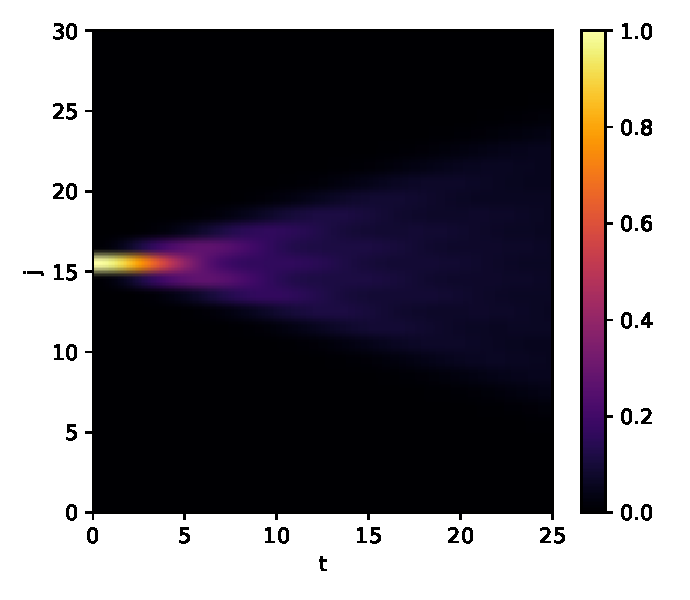
\includegraphics[width=\textwidth]{LaTeX/Plots/Ctj_g0.2_h0.0.pdf}
        \caption{The correlation $C(t,j)$.}
        \label{fig:4c_Correlation_g_0_2}
    \end{subfigure}
    \hfill % Adds horizontal space between the figures
    % Subfigure 2
    \begin{subfigure}[b]{0.32\textwidth}
        \centering
        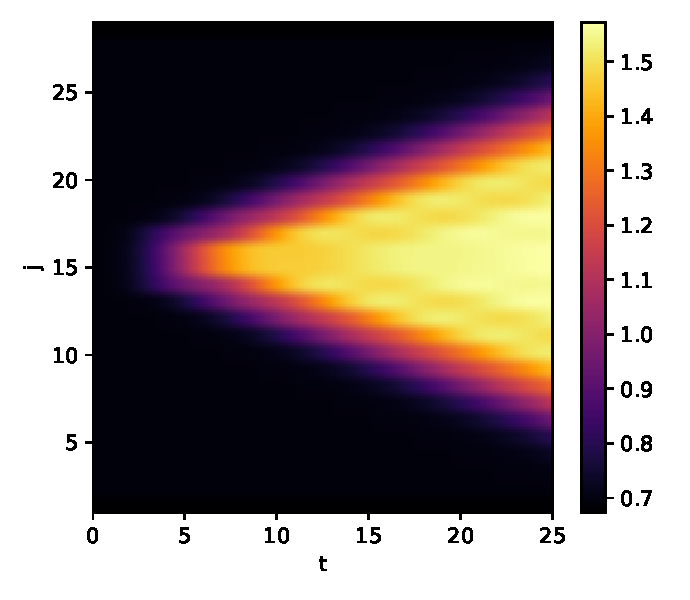
\includegraphics[width=\textwidth]{LaTeX/Plots/entropy_g0.2_h0.0.pdf}
        \caption{The v-N entanglement entropy $S(t)$.}
        \label{fig:4c_Entropy_g_0_2}
    \end{subfigure}
    \hfill % Adds horizontal space between the figures
    % Subfigure 3
    \begin{subfigure}[b]{0.32\textwidth}
        \centering
        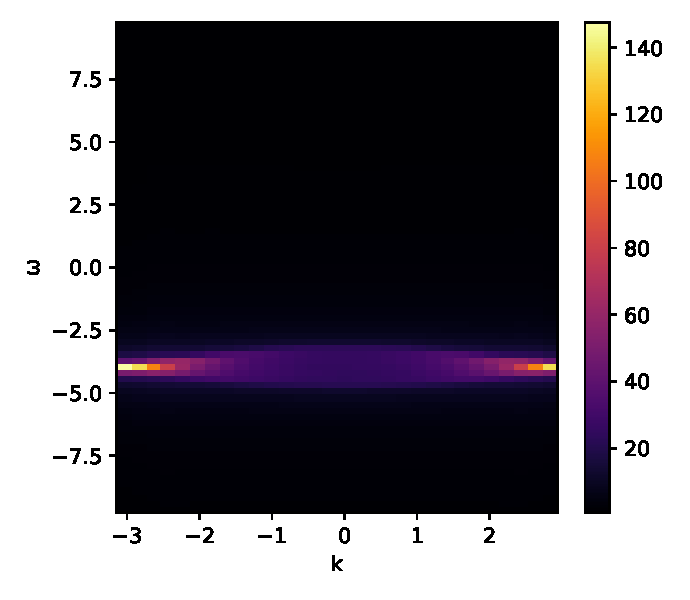
\includegraphics[width=\textwidth]{LaTeX/Plots/Skw_g0.2_h0.0.pdf}
        \caption{The spectrum $S(k,w)$.}
        \label{fig:4c_Spectrum_g_0_2}
    \end{subfigure}
    
    \caption{The correlation $C(t,j)$ (left), the entanglement entropy $S(t)$ (middle) and the spectrum $S(k,w)$ (right) for the case $g = 0.2$ and $h=0 $}
    \label{fig:4c_g_0_2}
\end{figure*}



\begin{figure*}[t]
    \centering
    % Subfigure 1
    \begin{subfigure}[b]{0.32\textwidth}
        \centering
        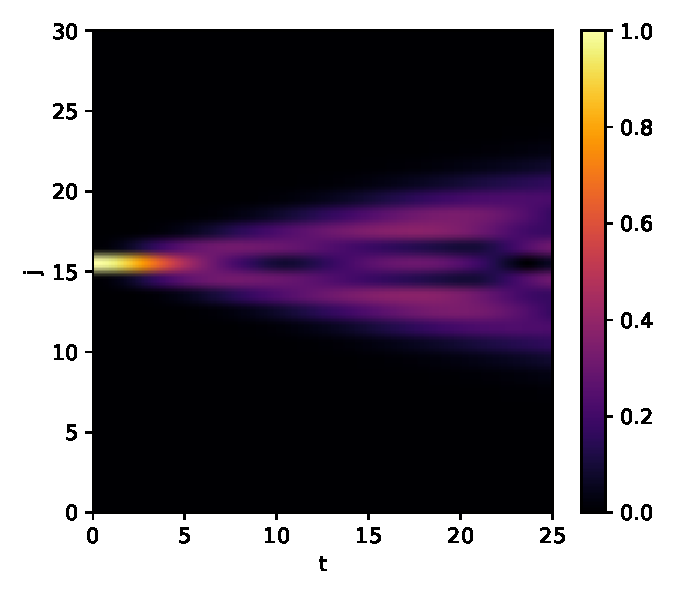
\includegraphics[width=\textwidth]{LaTeX/Plots/Ctj_g0.2_h0.1.pdf}
        \caption{The correlation $C(t,j)$.}
        \label{fig:4d_Correlation_g_0_2}
    \end{subfigure}
    \hfill % Adds horizontal space between the figures
    % Subfigure 2
    \begin{subfigure}[b]{0.32\textwidth}
        \centering
        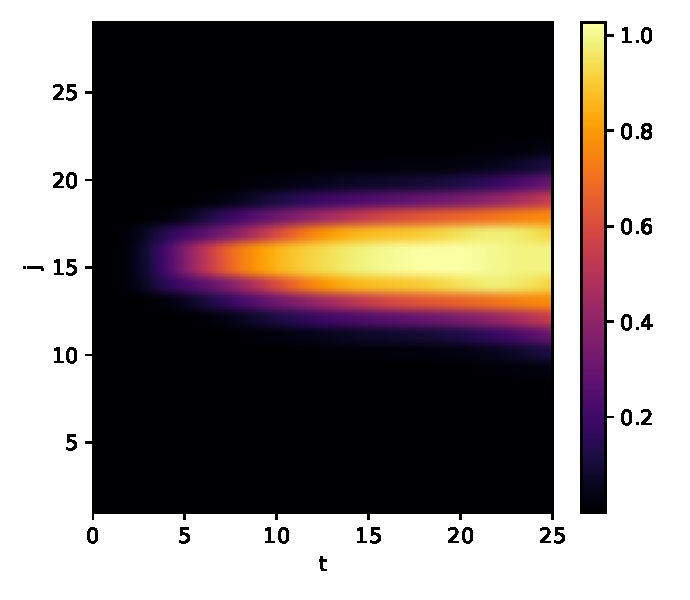
\includegraphics[width=\textwidth]{LaTeX/Plots/entropy_g0.2_h0.1.pdf}
        \caption{The v-N entanglement entropy $S(t)$.}
        \label{fig:4d_Entropy_g_0_2}
    \end{subfigure}
    \hfill % Adds horizontal space between the figures
    % Subfigure 3
    \begin{subfigure}[b]{0.32\textwidth}
        \centering
        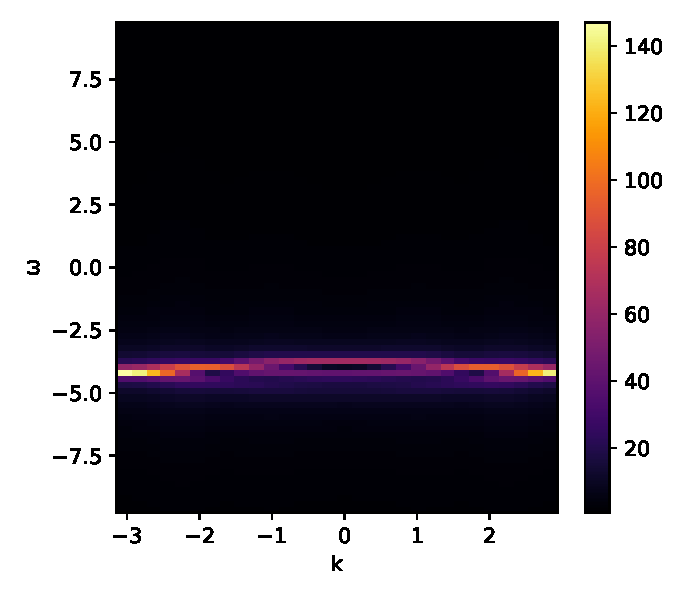
\includegraphics[width=\textwidth]{LaTeX/Plots/Skw_g0.2_h0.1.pdf}
        \caption{The spectrum $S(k,w)$.}
        \label{fig:4d_Spectrum_g_0_2}
    \end{subfigure}
    
    \caption{The correlation $C(t,j)$ (left), the entanglement entropy $S(t)$ (middle) and the spectrum $S(k,w)$ (right) for the case $g = 0.2$ and $h=0.1$}
    \label{fig:4d_g_0_2}
\end{figure*}



\begin{figure*}[t]
    \centering
    % Subfigure 1
    \begin{subfigure}[b]{0.32\textwidth}
        \centering
        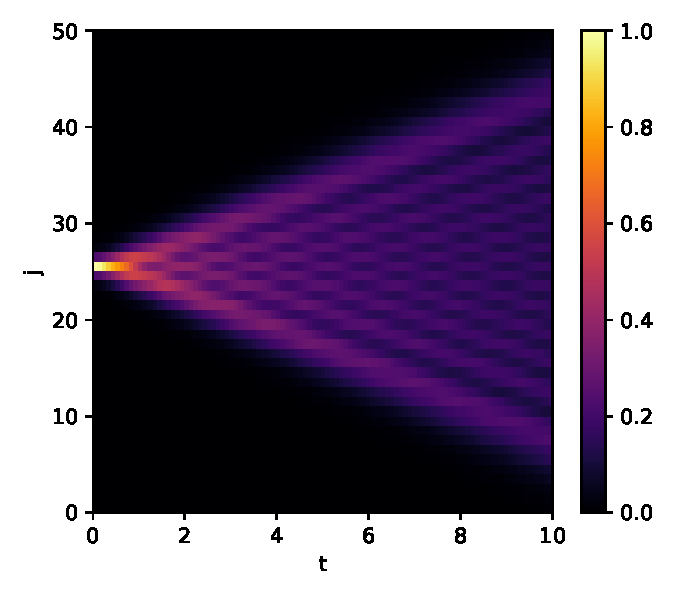
\includegraphics[width=\textwidth]{LaTeX/Plots/Ctj_g2.0_h0.0.pdf}
        \caption{The correlation $C(t,j)$.}
        \label{fig:4c_Correlation_g_2_0}
    \end{subfigure}
    \hfill % Adds horizontal space between the figures
    % Subfigure 2
    \begin{subfigure}[b]{0.32\textwidth}
        \centering
        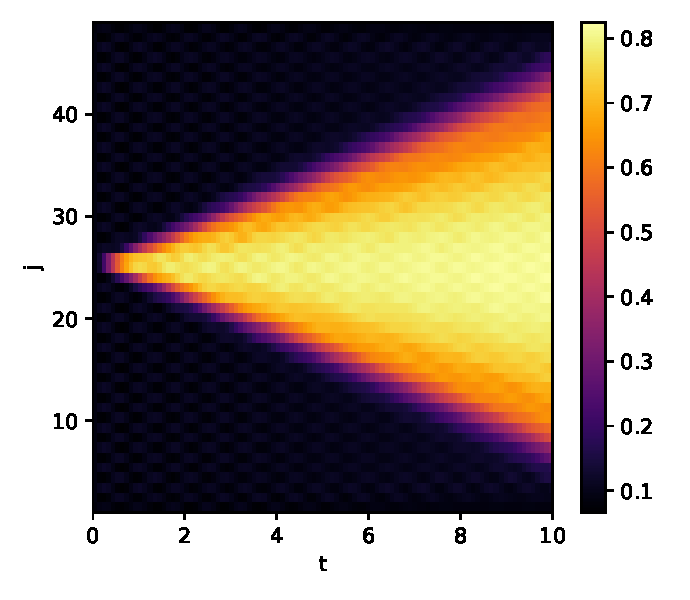
\includegraphics[width=\textwidth]{LaTeX/Plots/entropy_g2.0_h0.0.pdf}
        \caption{The v-N entanglement entropy $S(t)$.}
        \label{fig:4c_Entropy_g_2_0}
    \end{subfigure}
    \hfill % Adds horizontal space between the figures
    % Subfigure 3
    \begin{subfigure}[b]{0.32\textwidth}
        \centering
        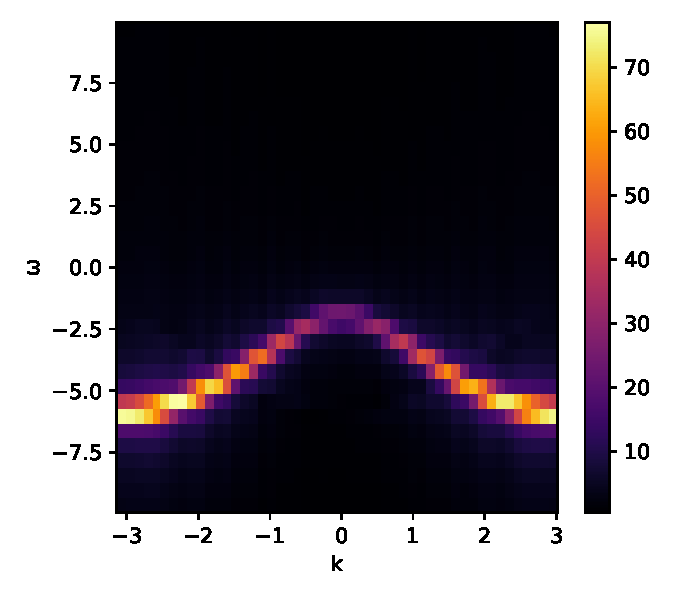
\includegraphics[width=\textwidth]{LaTeX/Plots/Skw_g2.0_h0.0.pdf}
        \caption{The spectrum $S(k,w)$.}
        \label{fig:4c_Spectrum_g_2_0}
    \end{subfigure}
    
    \caption{The correlation $C(t,j)$ (left), the entanglement entropy $S(t)$ (middle) and the spectrum $S(k,w)$ (right) for the case $g = 2.0$ and $h=0 $}
    \label{fig:4c_g_2_0}
\end{figure*}
